\documentclass[titlepage, 11pt]{article}
\usepackage{fixltx2e}
\usepackage{titlesec}

\titleformat*{\section}{\LARGE\bfseries}
\titleformat*{\subsection}{\Large\bfseries}
\titleformat*{\subsubsection}{\normalsize\bfseries}


\setlength{\oddsidemargin}{0.0in}
\setlength{\evensidemargin}{0.0in}
\setlength{\topmargin}{-0.25in}
\setlength{\headheight}{0in}
\setlength{\headsep}{0in}
\setlength{\textwidth}{6.5in}
\setlength{\textheight}{9.25in}
\setlength{\parindent}{0in}
\setlength{\parskip}{2mm}
\usepackage{listings, caption, color, xcolor, graphicx}
\pagestyle{plain}

\definecolor{gray}{rgb}{0.5,0.5,0.5}
\lstset{
basicstyle=\footnotesize\ttfamily,
breaklines=true,
captionpos=t,
numbers=left,
numbersep=5pt,
numberstyle=\tiny\color{gray},
tabsize=2,
title=\lstname,
language=C++,
keywordstyle=\bfseries\color{green!30!black},
commentstyle=\itshape\color{gray},
identifierstyle=\color{blue!40!black}
}

\captionsetup{labelformat=empty}

\title{\Huge ECS 158 Final Report: \\\LARGE combn() in Snow, OpenMP, and Thrust}
\date{}
\author{\huge Stefan Peterson\\\huge Bijan Agahi \\\huge Arjun Bharadwaj}

\begin{document}
\maketitle
\begin{abstract}
Parallel architectures are becoming increasingly prevalent in the modern world and as such have spawned multiple frameworks to assist with parallel programming, but these frameworks vary greatly in their implementation and performance. This paper takes a close look at three frameworks: R-Snow, OpenMP and Thrust. We took on the task of re-writing the combn() function found in R using each of these frameworks. We measure run times of these tests at different sizes and with varying inputs and levels of difficulty. In the end, we point out the strengths and weaknesses of each language as well as note on features which we, as programmers, find particularly useful or troublesome.
\end{abstract}
\tableofcontents
\newpage
\section{Introduction}
With the relatively recent introduction of widely available multi-processor CPUs in household computers, parallel programming has become a hot topic in the world of computer science. In particular, the graphics and games industry has driven the multithreaded programming style to the forefront of everyone's attention. Through the process of splitting up tasks and distributing those tasks to individual cores on the CPU or GPU, parallel processing in most cases can provide vast improvements in both performance and efficiency. OpenMP, R-Snow, and Thrust are three such parallel languages, and this paper aims to compare and contrast the strengths, weaknesses, and performance of each language.

\subsection{Setup for Benchmarks}
All tests for the purposes of this paper were run on Tetraat University of California, Davis. This computer consists of a 64-bit 8-core processor with 16 GB or RAM and an Intel Core i7-2600K CPU with a clock speed of 3.4 GHz and a cache size of 8192 KB. The machine was running release 19 of the linux distribution Fedora.



\section{combn() in OpenMP}
\subsection{Strategy}
For the OpenMP version of the combinations function, we decided to parallelize by dedicating each thread to a subsection of the problem. Each subsection corresponds to the group of combinations which begin with the same value. In [Appendix Graphic 2] we see all the possible combinations for a ${5 \choose 3}$. Those can be clumped into the three groups each beginning with 1, 2, or 3. \verb;Thread 1; will handle the computation of all combinations beginning with $1$, \verb;thread 2; will handle those beginning with $2$ and \verb;thread 3; will handle those beginning with $3$. Obviously this is not load balanced for small cases since \verb;thread 1; is doing significantly more work than the rest of the threads. When we get to larger problems, we use the built in dynamic scheduling of OpenMP to make an attempt at load balancing. If we had only 2 threads running on the above problem, \verb;thread 1; would still do its chunk of the computation, then \verb;thread 2; would do its and when it finishes (which should be before \verb;thread 1;) it grabs the next process to be executed.



\subsection{Implementation}

\begin{center}\textcolor{black!50}{All the references to code will be references to Appendix: A.1}\\ \end{center}
We decided to take a recursive approach to the implementation of the combinations function in C++. The core functionality of the program can be found on lines 23-33 in the method findCombs. This method takes in as its parameters 2 integers, a vector, and a 2d vector. Upon the first call of findCombs() the vector combination will already have been initialized to contain the first value in the combination (i.e. if we assume we are looking for the combination [1,2,3] the vector will be initialized to contain [1] and this is done on line 71 in the combn() function. From there the recursive algorithm will add the next number (i.e. combinations will now contain [1,2]) and then will call findCombs() recursively until the base case is met upon which the vector combination is pushed on to the 2D vector. When the recursion is done and the 2D vector contains all its possible combinations, the function vectorToArray() is called and the 2D vector is parsed and its values are added to the appropriate region of the global array. 


\subsection{Data}
\subsubsection{Graphic A1}
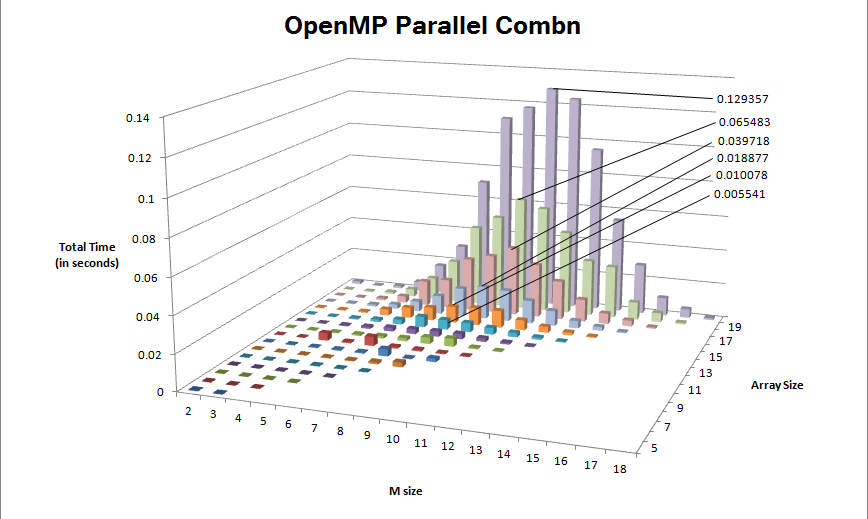
\includegraphics[scale = 0.5]{3D-OMP.png} \\
\subsubsection{Graphic A2}
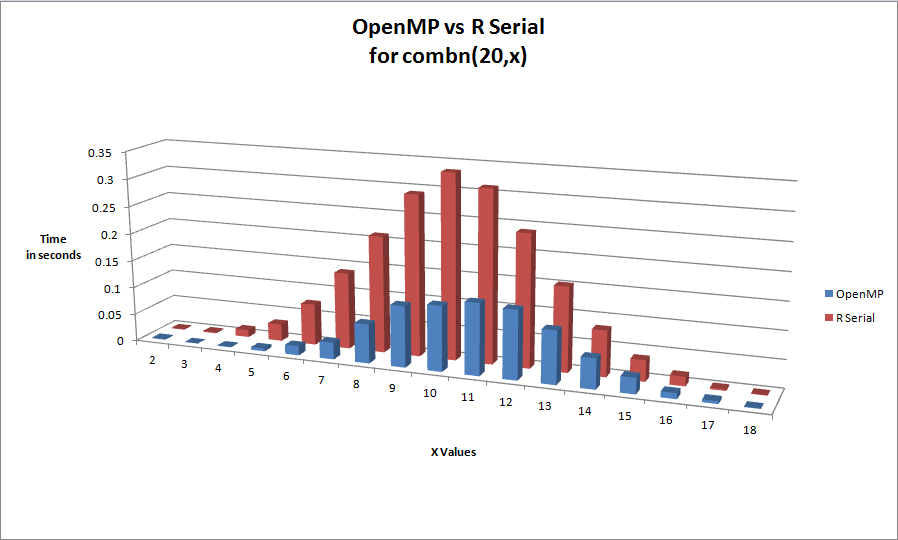
\includegraphics[scale = 0.5]{OMPvsR.png}

\subsection{Analysis}
Looking at \verb; Graphic A1; we can see that our implementation of $combn()$ in OpenMP follows the standard bell curve where given a value $x$, its maximum number of calculations and therefore its longest running time occurs when $m = \frac{x}{2}$. We can see this by looking at Pascal's Triangle [Appendix Graphic 1] which directly correlates to the problem of creating a list of combinations. Those values which lie at the center of each row, vertically down the middle, are those with the greatest value for that given row. These values correspond to ${x \choose m}$ where again $m = \frac{x}{2}$. When $combn()$ is passed these values this is when we see the greatest running time for the function. \\

Looking at \verb; Graphic A2; we can see that our implementation of $combn()$ is on average 2-3 times faster than the serial built in version provided in the utils package of the R library. This is to be expected since we are able to generate combinations in parallel speed up could be further improved by taking our approach of parallelization further down and assigning tasks recursively.

\section{combn() in Thrust}

\subsection{Strategy}

\subsection{Implementation}
\begin{center}\textcolor{black!50}{All the references to code will be references to Appendix: A.2}\\ \end{center}


\subsection{Data}
\subsubsection{Graphic B1}
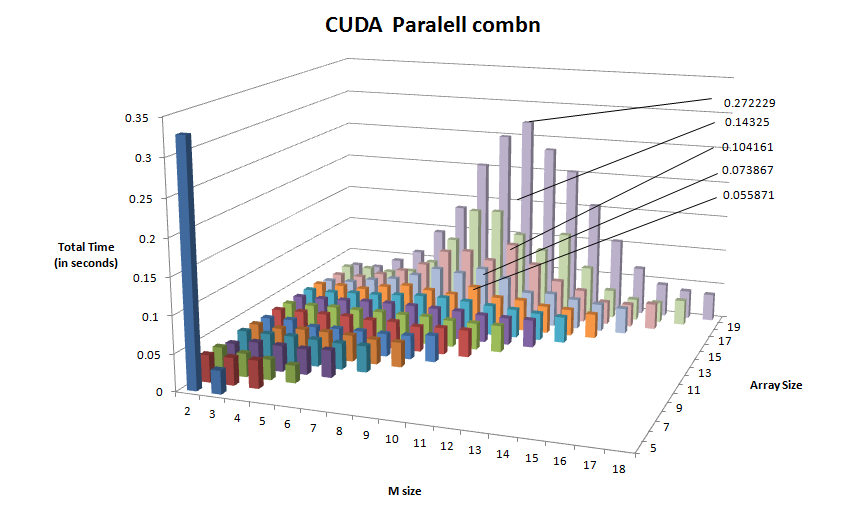
\includegraphics[scale = 0.5]{3D-Thrust.png} \\
\subsubsection{Graphic B2}
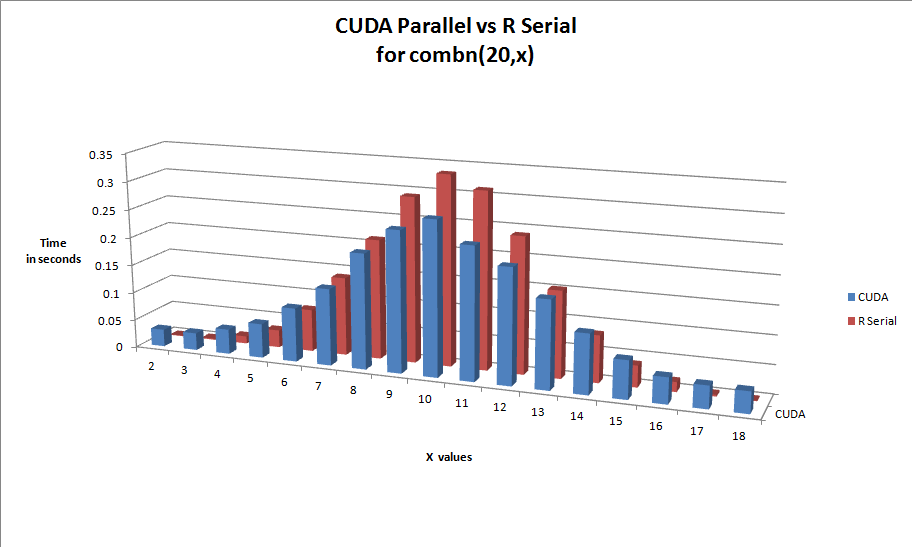
\includegraphics[scale = 0.5]{ThrustvsR.png}

\subsection{Analysis}
Looking at \verb; Graphic B1; we can see that our implementation of $combn()$ in Thrust follows a similar bell curve to that of the one in our OpenMP implementation. There is a large difference though, in that in the Thrust implementation, you never see a close to zero time operation like you do in a lot of the cases for the OpenMP. This is due to the fact that Thrust operates on the GPU and as such has to transfer data both to and from the GPU before and after computation. This travel time between CPU and GPU accounts for the "baseline" being roughly .025 seconds meaning no operations ever run faster than this.

Looking at \verb; Graphic B2; we can see that our implementation of $combn()$ in Thrust outperforms the serial built in version provided in the utils package of the R library for values where given an x and m for ${x \choose m}$ the value of m is roughly $\frac{x}{4} < m < \frac{3x}{4}$. So for values which are generally computation heavy, the Thrust implementation is faster and provides performance gains, but for less computation heavy problems, the transport cost is not worth the small speed up of the parallelization.

\section{combn() in R-Snow}

\subsection{Strategy}

\subsection{Implementation}


\subsection{Data}

\subsection{Analysis}




\section{Conclusion}
Overall, the run times achieved by parallelization seem to have improvements, significantly so in the OpenMP implementation. Each run time seems to have its own pros and cons. Thrust provided strong performance gains over the serial version but required the overhead of having to transport data on a slow connection from the CPU to GPU. The algorithm we used for parallel computation was also probably not the most efficient and we could have seen even better gains in performance, but with Thrust this still doesn't matter for "easy" computations where transport time far exceeds computation time. OpenMP runs the fastest of the three and this is due to the fact that both our algorithm for OpenMP was probably the most efficient of our three algorithms and that there is not overhead necessary before beginning the computations. The biggest hurdle with our OpenMP implementation is making sure that it is load balanced.


\section{Bibliography}


\pagebreak
\appendix
\section{Appendix: Code}
\subsection{combn() --- OpenMP implementation}
\lstinputlisting[language=C++]{combnOpenMP.cpp}
This is a recursive implementation of the combinations function. Here we used \verb; #pragma omp parallel for schedule(dynamic); on line 67 to help load balance the parallelization of the threading.  \\
\subsection{combn() --- Thrust implementation}
\lstinputlisting[language=C++]{combn.cu}
This code uses the built in stl function $next_permutation()$ .... ARJUN FINISH THIS PLEASE \\


There are also a variety of files specific for testing purposes included in the submitted .tar file.

\section{Appendix: Graphics}
\subsection{Graphic D1}
\begin{center}
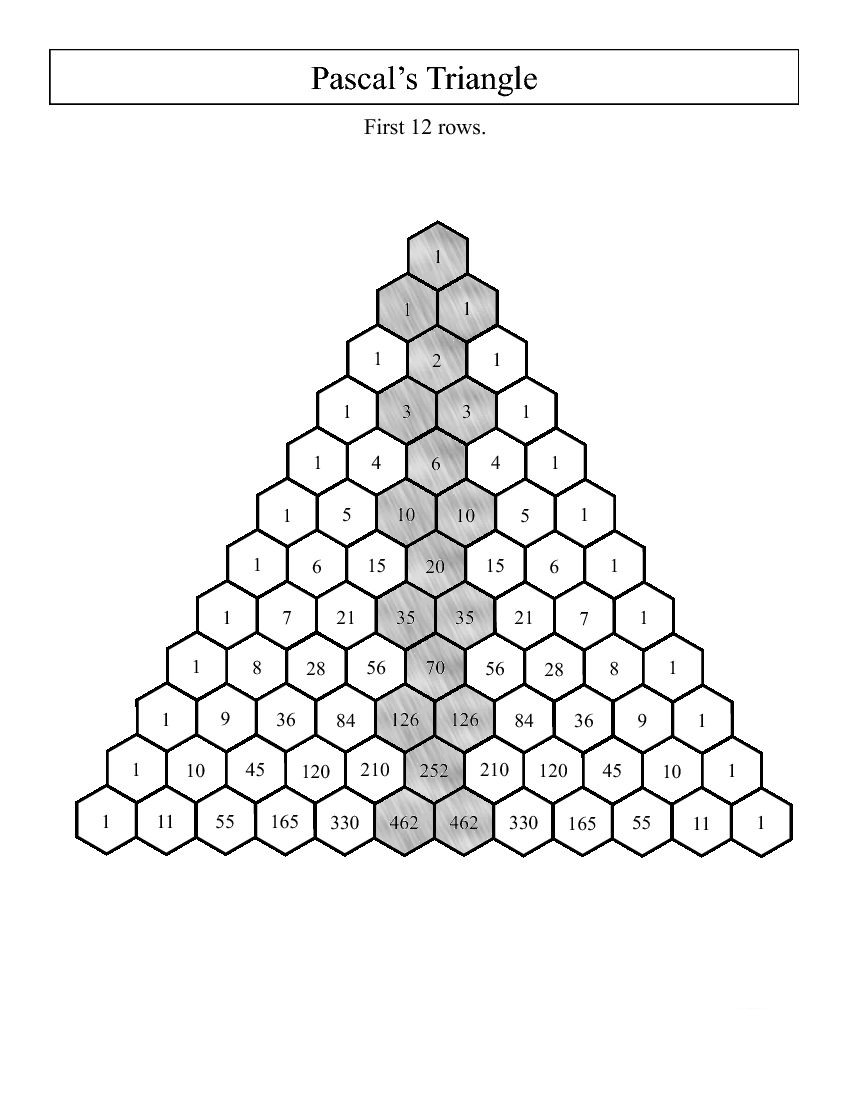
\includegraphics[scale = 0.4]{pascals-triangle-vert.jpg} \\
\end{center}

\subsection{Graphic D2}
\begin{center}
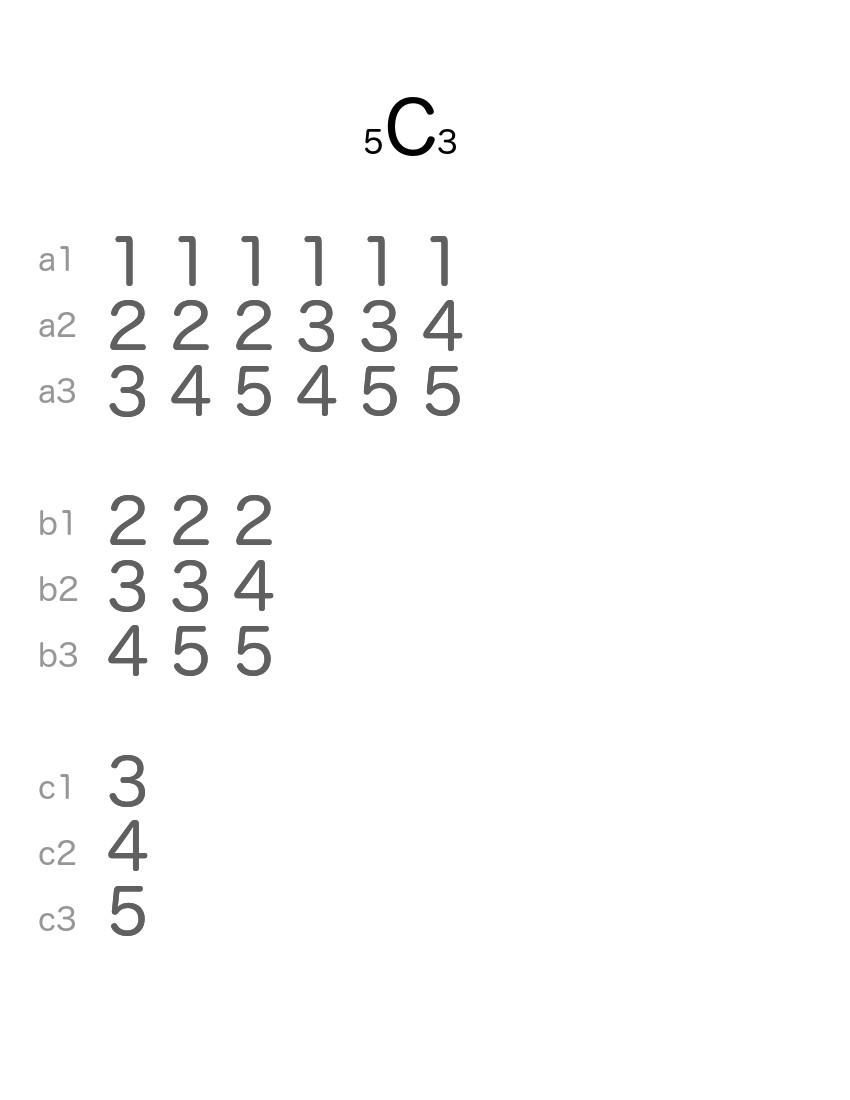
\includegraphics[scale = 0.25]{5Choose3.jpg} \\
\end{center}

\newpage
\section{Appendix: Member Contributions}

\textbf{Stefan Peterson}
\begin{itemize}
	\item \LaTeX{} Formatting, editing
	\item OpenMP implementation
	\item OpenMP write-up
	\item Abstract
	\item Introduction
	\item Conclusion
	\item Relevant research
\end{itemize}

\textbf{Bijan Agahi}
\begin{itemize}
	\item R-Snow implementation
	\item Experiment data collection
	\item Test scripting
	\item Graphing in R, tabling
	\item Relevant research
\end{itemize}

\textbf{Arjun Bharadwaj}
\begin{itemize}
	\item Thrust implementation
	\item Relevant research
\end{itemize}

\end{document}